% --------------------------------------------------------------------------- %
% Poster for the ECCS 2011 Conference about Elementary Dynamic Networks.      %
% --------------------------------------------------------------------------- %
% Created with Brian Amberg's LaTeX Poster Template. Please refer for the     %
% attached README.md file for the details how to compile with `pdflatex`.     %
% --------------------------------------------------------------------------- %
% $LastChangedDate:: 2011-09-11 10:57:12 +0200 (V, 11 szept. 2011)          $ %
% $LastChangedRevision:: 128                                                $ %
% $LastChangedBy:: rlegendi                                                 $ %
% $Id:: poster.tex 128 2011-09-11 08:57:12Z rlegendi                        $ %
% --------------------------------------------------------------------------- %
\documentclass[a0paper,portrait]{baposter}

\usepackage{relsize}		% For \smaller
\usepackage{url}			% For \url
\usepackage{epstopdf}	% Included EPS files automatically converted to PDF to include with pdflatex
\usepackage{cite}
\usepackage{xcolor}

%%% Global Settings %%%%%%%%%%%%%%%%%%%%%%%%%%%%%%%%%%%%%%%%%%%%%%%%%%%%%%%%%%%

\graphicspath{{pix/}}	% Root directory of the pictures 
\tracingstats=2			% Enabled LaTeX logging with conditionals

%%% Color Definitions %%%%%%%%%%%%%%%%%%%%%%%%%%%%%%%%%%%%%%%%%%%%%%%%%%%%%%%%%

\definecolor{bordercol}{RGB}{40,40,40}
\definecolor{headercol1}{RGB}{186,215,230}
\definecolor{headercol2}{RGB}{80,80,80}
\definecolor{headerfontcol}{RGB}{0,0,0}
\definecolor{boxcolor}{RGB}{186,215,230}

%%%%%%%%%%%%%%%%%%%%%%%%%%%%%%%%%%%%%%%%%%%%%%%%%%%%%%%%%%%%%%%%%%%%%%%%%%%%%%%%
%%% Utility functions %%%%%%%%%%%%%%%%%%%%%%%%%%%%%%%%%%%%%%%%%%%%%%%%%%%%%%%%%%

%%% Save space in lists. Use this after the opening of the list %%%%%%%%%%%%%%%%
\newcommand{\compresslist}{
	\setlength{\itemsep}{1pt}
	\setlength{\parskip}{0pt}
	\setlength{\parsep}{0pt}
}

%%%%%%%%%%%%%%%%%%%%%%%%%%%%%%%%%%%%%%%%%%%%%%%%%%%%%%%%%%%%%%%%%%%%%%%%%%%%%%%
%%% Document Start %%%%%%%%%%%%%%%%%%%%%%%%%%%%%%%%%%%%%%%%%%%%%%%%%%%%%%%%%%%%
%%%%%%%%%%%%%%%%%%%%%%%%%%%%%%%%%%%%%%%%%%%%%%%%%%%%%%%%%%%%%%%%%%%%%%%%%%%%%%%

\begin{document}
\typeout{Poster rendering started}

%%% Setting Background Image %%%%%%%%%%%%%%%%%%%%%%%%%%%%%%%%%%%%%%%%%%%%%%%%%%
\background{
	\begin{tikzpicture}[remember picture,overlay]%
	\draw (current page.north west)+(-2em,2em) node[anchor=north west]
	{\includegraphics[height=1.1\textheight]{background}};
	\end{tikzpicture}
}

%%% General Poster Settings %%%%%%%%%%%%%%%%%%%%%%%%%%%%%%%%%%%%%%%%%%%%%%%%%%%
%%%%%% Eye Catcher, Title, Authors and University Images %%%%%%%%%%%%%%%%%%%%%%
\begin{poster}{
	grid=false,
	% Option is left on true though the eyecatcher is not used. The reason is
	% that we have a bit nicer looking title and author formatting in the headercol
	% this way
	%eyecatcher=false, 
	borderColor=bordercol,
	headerColorOne=headercol1,
	headerColorTwo=headercol2,
	headerFontColor=headerfontcol,
	% Only simple background color used, no shading, so boxColorTwo isn't necessary
	boxColorOne=boxcolor,
	headershape=roundedright,
	headerfont=\Large\sf\bf,
	textborder=rectangle,
	background=user,
	headerborder=open,
  boxshade=plain
}
%%% Eye Cacther %%%%%%%%%%%%%%%%%%%%%%%%%%%%%%%%%%%%%%%%%%%%%%%%%%%%%%%%%%%%%%%
{
	Eye Catcher, empty if option eyecatcher=false - unused
}
%%% Title %%%%%%%%%%%%%%%%%%%%%%%%%%%%%%%%%%%%%%%%%%%%%%%%%%%%%%%%%%%%%%%%%%%%%
{\sf\bf
A Soft Coarse-Grained Reconfigurable Array Based High-level Synthesis Methodology: Promoting Design 
Productivity and Exploring Extreme FPGA Frequency
}
%%% Authors %%%%%%%%%%%%%%%%%%%%%%%%%%%%%%%%%%%%%%%%%%%%%%%%%%%%%%%%%%%%%%%%%%%
{
	\vspace{1em} Cheng Liu, Colin Yu Lin, Hayden Kwok-Hay So\\
	{\smaller liucheng@eee.hku.hk, linyu@eee.hku.hk, hso@eee.hku.hk}
}
%%% Logo %%%%%%%%%%%%%%%%%%%%%%%%%%%%%%%%%%%%%%%%%%%%%%%%%%%%%%%%%%%%%%%%%%%%%%
{
% The logos are compressed a bit into a simple box to make them smaller on the result
% (Wasn't able to find any bigger of them.)
\setlength\fboxsep{0pt}
\setlength\fboxrule{0pt}
	\fbox{
		\begin{minipage}{12em}
			\includegraphics[width=12em,height=12em]{hkulogo}
		\end{minipage}
	}
}

\headerbox{Background and Motivation}{name=problem,column=0,row=0}{
Compared to the use of a typical software development flow, the productivity of developing FPGA-based compute
applications remains much lower[1]. There are two reasons for this.
\begin{itemize}
\item Current high-level synthesis (HLS) tools seldom help to reduce the lengthy low-level FPGA implementation process.
\item High-level application developers often lack the intimate hardware engineering experience to achieve high performance on FPGAs.
%Although the use of high-level synthesis (HLS) tools may partly alleviate this
%shortcoming, the lengthy low-level FPGA implementation process remains a major obstacle to high productivity computing,
%limiting the number of compile-debug-edit cycles per day. Furthermore, high-level application developers often
%lack the intimate hardware engineering experience that is needed to achieve high performance on FPGAs, therefore
%undermining their usefulness as accelerators.
\end{itemize}
}

\headerbox{SCGRA}{name=scgra,column=0,below=problem}{
The implementation of the SCGRA has a significant impact on the overall performance. An instance of such SCGRA design is thus presented
to demonstrate the feasibility of producing high performance gateware without incurring long compilation time. One PE of the SCGRA is 
shown in the Figure below.

\setlength\fboxsep{0pt}
\setlength\fboxrule{0pt}

\begin{center}
\fcolorbox{white}{white!100}{
\fbox{
\begin{minipage}{19em}
\begin{center}
\includegraphics[width=0.9\linewidth]{pe}
\end{center}
\end{minipage}
}
}
\end{center}
}

\headerbox{Conclusion}{name=conclusion, column=0,below=scgra}{
\begin{itemize}
\item By using SCGRA as an intermediate compile step, the lengthy low-level implementation tool 
flow is reduced to a relatively rapid operation scheduling problem, which contributes directly 
to higher application designers' productivity.

\item Implementation with close to maximum clock frequency resulting from the highly regular structure 
of the SCGRA, in combination with an in-house scheduler that can effectively schedule operation 
to overlap with pipeline latencies guarantee the overall high performance.
\end{itemize}
}

\headerbox{References}{name=references,column=0,below=conclusion,above=bottom}{
%\smaller
\vspace{-0.4em}
%\bibliographystyle{plain}
%\bibliography{refs}
\bibliographystyle{plain}				
\renewcommand{\section}[2]{\vskip 0.05em}
\begin{thebibliography}{1}			
\itemsep=-0.01em				
\setlength{\baselineskip}{0.4em}
\bibitem{ref1} Lavin, C. and Padilla, M. and Ghosh, S. and Nelson, B. and Hutchings, B. and Wirthlin, M., Using hard macros to reduce FPGA compilation time, International conference on Field Programmable Logic and Applications, 2010
\bibitem{ref2} The LLVM compiler framework, http://llvm.org
\bibitem{ref3} Cong, J. and Liu, B. and Neuendorffer, S. and Noguera, J. and Vissers, K. and Zhang, Z., High-level synthesis for FPGAs: From prototyping to deployment, IEEE Transactions on Computer-Aided Design of Integrated Circuits and Systems, 2011
\end{thebibliography}

} 

\headerbox{Proposed Design Methodology}{name=designmethod,span=2,column=1,row=0}{
To Address the productivity and performance problems, a HLS methodology that utilizes soft coarse-grained reconfigurable
arrays (SCGRAs) as an intermediate compilation step as shown in the figure below is presented. Instead of compiling high-level applications directly
to circuits, the compilation process is reduced to an operation scheduling task targeting the SCGRA.

\vspace{-0.2em}
\setlength\fboxsep{0pt}
\setlength\fboxrule{0pt}
\begin{center}
\fcolorbox{white}{white!100}{
    \fbox{
        \begin{minipage}{42em}
        \begin{center}
        \includegraphics[width=0.98\linewidth]{designflow}
        \end{center}
        \end{minipage}
    }
}
\end{center}

}

\headerbox{Experiment setup}{name=setup,column=1,below=designmethod}{
We take 5 computation kernels including matrix multiply (MM), fast Fourier transform (FFT), discrete
convolution (CONV), advanced encryption standard (AES) and Viterbi decoder (VD) as our benchmark.

All runtimes were obtained on a Linux workstation with an
Intel(R) Xeon(R) CPU E5345 and 8GB of RAM. All the implementations targeted Xilinx Virtex6 FPGA (xc6vlx240t784-
1). The proposed HLS methodology employed LLVM v3.1
and clang v3.1 [2] for C program compiling and PlanAhead
v13.4 for the SCGRA implementations. As for the direct
mapping methodology, AutoESL 2011.4.2 [3] was taken as a
representative.
}

\headerbox{Experiment-1}{name=experiment1,column=1,below=setup,above=bottom}{
AutoESL includes two steps: AutoESL synthesis and AutoESL implementation. The proposed HLS methodology bypasses 
the lengthy low-level implementation steps and simply needs three high-level steps: LLVM compiling, SCGRA 
scheduling and bitstream integration. As shown in the figure below, it is generally 10X-100X faster.

\begin{center}
\includegraphics[width=0.92\linewidth]{designtime}
\end{center}

}

\headerbox{Experiment-2}{name=experiment2,column=2,below=designmethod,above=bottom}{
The figure below displays the implementation frequency. It is clear that the implementations using 
the proposed HLS methodology for all the kernels are much higher than those using AutoESL. 

\begin{center}
\includegraphics[width=0.92\linewidth]{impl_freq}
\end{center}

The following figure shows the simulation performance. The proposed design methodology outperforms
AutoESL for most of the kernels. 

\begin{center}
\includegraphics[width=0.92\linewidth]{sim_perf}
\end{center}

With both implementation frequency and simulation performance given in previous two figures, 
the proposed design methodology achieved 0.8-21x times speedup in the application run time.

\begin{center}
\includegraphics[width=0.92\linewidth]{real_perf}
\end{center}

}

\end{poster}
\end{document}
